%%%%%%%%%
\section{基本运算符}

\subsection{赋值运算符}
\begin{frame}[fragile]\ft{\subsecname}
\begin{lstlisting}[language=c,backgroundcolor=\color{red!10}]
  int n; 
  n = 2016;
\end{lstlisting} \pause 

\begin{itemize}
\item 在C中,\lstinline|=| 是一个赋值运算符(assignment operator),不表示“相等”。\\[0.15in]
\item 请读成“将值2016赋给变量n”,而不是“n等于2016”。\\[0.15in]
\item 赋值运算符的动作是从右到左。
\end{itemize}

\end{frame}

\begin{frame}[fragile]\ft{\subsecname}
\begin{lstlisting}[language=c,backgroundcolor=\color{red!10}]
  i = i + 1;
\end{lstlisting} \pause 
\begin{figure}
\centering
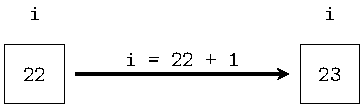
\includegraphics[width=3in]{ch05/images/assign.pdf}
\end{figure}
\end{frame}

\begin{frame}[fragile]\ft{\subsecname}
以下语句没有意义:
\begin{lstlisting}[language=c,backgroundcolor=\color{red!10}]
  2016 = n;
\end{lstlisting} 	
因不能将一个值赋给常量。
\end{frame}

\begin{frame}[fragile]\ft{\subsecname}
\begin{enumerate}
\item 左值: 指向内存位置的表达式称为\red{左值表达式}。\\[0.4cm]
\item[] 左值可以是变量名或表达式,但表达式必须表示的是个内存位置。\\[0.4cm]
\item 右值: 存储在内存中某些位置的数值。\\[0.4cm]
\item 操作数:运算符操作的对象。
\end{enumerate}
\end{frame}


\begin{frame}[fragile]\ft{\subsecname}
\lstinputlisting[language=c,frame=single,numbers=left]{ch05/code/AssignOpThree.c}
\end{frame}


\begin{frame}[fragile]\ft{\subsecname}
\begin{lstlisting}[backgroundcolor=\color{red!10}]    
$ gcc AssignOpThree.c
$ ./a.out
a = 10, b = 10, c = 10  
\end{lstlisting}

\pause \vspace{.1in}

赋值的过程是从右到左的。先将10赋给c,再将c的值赋给b,最后将b的值赋给a。
\end{frame}

\subsection{加减运算符}
\begin{frame}[fragile]\ft{\subsecname}
加法运算符(addition operator)将其两侧的操作数进行相加。 \vspace{1em}

\begin{lstlisting}
printf("%d", 4+20);
\end{lstlisting}
\vspace{1em}

两个操作数可以是变量,也可以是常量,如
\begin{lstlisting}
c = a + b;
\end{lstlisting}
\end{frame}
 
\begin{frame}[fragile]\ft{\subsecname}
减法运算符(subtraction operator)将它前面的数减去后面的数。\vspace{1em}

\begin{lstlisting}
b = 20.0 - 200.0;
\end{lstlisting}
\vspace{1em}

\lstinline|+| 和 \lstinline|-| 运算符被称为双目运算符,因为它们都需要两个操作数。
\end{frame}


\begin{frame}[fragile]\ft{\subsecname}
\lstinline|+| 和 \lstinline|-| 也可以用作单目运算符。
\vspace{1em}

\begin{lstlisting}[language=c,backgroundcolor=\color{red!10}]
a = -1;
b = -a;
\end{lstlisting}
此时 \lstinline|-| 表示负号,用于指示或改变一个值的符号。
\vspace{1em}

C99引入了单目运算符 \lstinline|+|,它不改变操作数的值或符号:
\begin{lstlisting}[language=c,backgroundcolor=\color{red!10}]
a = +1;
\end{lstlisting}
\end{frame}

\subsection{乘法运算符}
\begin{frame}[fragile]\ft{\subsecname}
\begin{lstlisting}[language=c,backgroundcolor=\color{red!10}]
  mile = 1.6 * km;
\end{lstlisting}
\vspace{1em}

\red{注意:C没有提供计算平方的运算符。}
\end{frame}


\begin{frame}[fragile]\ft{\subsecname}

\lstinputlisting[language=c,numbers=left]{ch05/code/squares.c}
\end{frame}


\begin{frame}[fragile]\ft{\subsecname}
\begin{lstlisting}[backgroundcolor=\color{red!10}]
$ gcc squares.c
$ ./a.out 
   1^2 =      1
   2^2 =      4
   3^2 =      9
   4^2 =     16
   5^2 =     25
   6^2 =     36
   7^2 =     49
   8^2 =     64
   9^2 =     81
\end{lstlisting}
\end{frame}



\subsection{除法运算符}
\begin{frame}[fragile]\ft{\subsecname}
  \lstinputlisting[language=c,numbers=left]{ch05/code/divide.c}    
\end{frame}
\begin{frame}[fragile]\ft{\subsecname}
\begin{lstlisting}[backgroundcolor=\color{red!10}]
$ gcc divide.c
$ ./a.out  
3 / 4 = 0
6 / 3 = 2
7 / 4 = 1
7. / 4. = 1.75
7. / 4  = 1.75
\end{lstlisting}    
\end{frame}




\begin{frame}[fragile]\ft{\subsecname}
\begin{itemize}
\item 整数相除,其结果的小数部分会被丢弃,称之为截尾。\\[0.1in]
\item 浮点数相除会得到一个浮点数结果。\\[0.1in]
\item C允许用一个整数去除浮点数,其结果也是浮点数。在此情况下,做除法运算之前会将整数化为浮点数。
\end{itemize}
\end{frame}

\subsection{运算符优先级}
\begin{frame}[fragile]\ft{\subsecname}
\begin{table}
\centering
\begin{tabular}{c|c} \hline
运算符& 结合性\\\hline\hline
\lstinline|()| & 从左到右 \\\hline
\lstinline|+, -|(单目运算符) & 从右到左\\\hline
\lstinline|*, /| & 从左到右 \\\hline
\lstinline|+, -|(双目运算符) & 从左到右 \\\hline
\lstinline|=| & 从右到左\\\hline
\end{tabular}
\end{table}
\end{frame}


\begin{frame}[fragile]\ft{\subsecname}
\begin{lstlisting}[frame=no,backgroundcolor=\color{red!10}]
y = 6 * 12 + 5 * 20;
\end{lstlisting}

\rule{\textwidth}{1mm}\pause 

\begin{itemize}
\item 根据优先级规定,两个乘法运算在加法运算之前进行。\\[0.1in]
\item 至于两个乘法运算谁先进行,C将此选择权留给实现者。
\end{itemize}

\end{frame}

\begin{frame}[fragile]\ft{\subsecname}
\begin{lstlisting}[frame=no,backgroundcolor=\color{red!10}]
y = 12 / 3 * 2;
\end{lstlisting}
\rule{\textwidth}{1mm}\pause 

\begin{itemize}
\item 结合规则适用于\red{共享同一操作数的运算符}。\\[0.1in]
\item  \lstinline|/| 和 \lstinline|*| 优先级相同,它们共享操作数3,按“从左到右”的结合原则,应该先算12/3。
\end{itemize}
\end{frame}

\begin{frame}[fragile]\ft{\subsecname}
\lstinputlisting[language=c,numbers=left,backgroundcolor=\color{red!10}]{ch05/code/rules.c}

\pause \vspace{.1in}

\begin{lstlisting}[backgroundcolor=\color{red!10}]
$ gcc rules.c
$ ./a.out  
b = -23
\end{lstlisting}
\end{frame}

\begin{frame}[fragile]\ft{\subsecname}
\begin{lstlisting}[numbers=left,backgroundcolor=\color{red!10}]
b = a = -(2 + 5) * 6 + (4 + 3 * (2 + 3));
b = a = -7 * 6 + (4 + 3 * (2 + 3));
b = a = -7 * 6 + (4 + 3 * 5);
b = a = -7 * 6 + (4 + 15);
b = a = -7 * 6 + 19;
b = a = -42 + 19;
b = a = -23;
b = -23;
\end{lstlisting}
\end{frame}

